\documentclass{article}
\usepackage{graphicx} % Required for inserting images

% header

%% natbib
\usepackage{natbib}
\bibliographystyle{plain}

%% comment
\usepackage{comment}

% no automatic indentation
\usepackage{indentfirst}

% manually indent
\usepackage{xargs} % \newcommandx
\usepackage{calc} % calculation
\newcommandx{\tab}[1][1=1]{\hspace{\fpeval{#1 * 10}pt}}
% \newcommand[number of parameters]{output}
% \newcommandx[number of parameters][parameter index = x]{output}
% use parameter index = x to substitute the default argument
% use #1, #2, ... to get the first, second, ... arguments
% \tab for indentation
% \tab{2} for for indentation twice

% note
\newcommandx{\note}[1]{\textit{\textcolor{red}{#1}}}
\newcommand{\todo}{\note{TODO}}
% \note{TODO}

%% math package
\usepackage{amsfonts}
\usepackage{amsmath}
\usepackage{amssymb}
\usepackage{tikz-cd}
\usepackage{mathtools}
\usepackage{amsthm}

%% operator
\DeclareMathOperator{\tr}{tr}
\DeclareMathOperator{\diag}{diag}
\DeclareMathOperator{\sign}{sign}
\DeclareMathOperator{\grad}{grad}
\DeclareMathOperator{\curl}{curl}
\DeclareMathOperator{\Div}{div}
\DeclareMathOperator{\card}{card}
\DeclareMathOperator{\Span}{span}
\DeclareMathOperator{\real}{Re}
\DeclareMathOperator{\imag}{Im}
\DeclareMathOperator{\supp}{supp}
\DeclareMathOperator{\im}{im}
\DeclareMathOperator{\aut}{Aut}
\DeclareMathOperator{\inn}{Inn}
\DeclareMathOperator{\Char}{char}
\DeclareMathOperator{\Sylow}{Syl}
\DeclareMathOperator{\coker}{coker}
\DeclareMathOperator{\inc}{in}
\DeclareMathOperator{\Sd}{Sd}
\DeclareMathOperator{\Hom}{Hom}
\DeclareMathOperator{\interior}{int}
\DeclareMathOperator{\ob}{ob}
\DeclareMathOperator{\Set}{Set}
\DeclareMathOperator{\Top}{Top}
\DeclareMathOperator{\Meas}{Meas}
\DeclareMathOperator{\Grp}{Grp}
\DeclareMathOperator{\Ab}{Ab}
\DeclareMathOperator{\Ch}{Ch}
\DeclareMathOperator{\Fun}{Fun}
\DeclareMathOperator{\Gr}{Gr}
\DeclareMathOperator{\End}{End}
\DeclareMathOperator{\Ad}{Ad}
\DeclareMathOperator{\ad}{ad}
\DeclareMathOperator{\Bil}{Bil}
\DeclareMathOperator{\Skew}{Skew}
\DeclareMathOperator{\Tor}{Tor}
\DeclareMathOperator{\Ho}{Ho}
\DeclareMathOperator{\RMod}{R-Mod}
\DeclareMathOperator{\Ev}{Ev}
\DeclareMathOperator{\Nat}{Nat}
\DeclareMathOperator{\id}{id}
\DeclareMathOperator{\Var}{Var}
\DeclareMathOperator{\Cov}{Cov}
\DeclareMathOperator{\RV}{RV}
\DeclareMathOperator{\rank}{rank}

%% pair delimiter
\DeclarePairedDelimiter{\abs}{\lvert}{\rvert}
\DeclarePairedDelimiter{\inner}{\langle}{\rangle}
\DeclarePairedDelimiter{\tuple}{(}{)}
\DeclarePairedDelimiter{\bracket}{[}{]}
\DeclarePairedDelimiter{\set}{\{}{\}}
\DeclarePairedDelimiter{\norm}{\lVert}{\rVert}

%% theorems
\newtheorem{axiom}{Axiom}
\newtheorem{definition}{Definition}
\newtheorem{theorem}{Theorem}
\newtheorem{proposition}{Proposition}
\newtheorem{corollary}{Corollary}
\newtheorem{lemma}{Lemma}
\newtheorem{remark}{Remark}
\newtheorem{claim}{Claim}
\newtheorem{problem}{Problem}
\newtheorem{assumption}{Assumption}
\newtheorem{example}{Example}
\newtheorem{exercise}{Exercise}

%% empty set
\let\oldemptyset\emptyset
\let\emptyset\varnothing

\newcommand\eps{\epsilon}

% mathcal symbols
\newcommand\Tau{\mathcal{T}}
\newcommand\Ball{\mathcal{B}}
\newcommand\Sphere{\mathcal{S}}
\newcommand\bigO{\mathcal{O}}
\newcommand\Power{\mathcal{P}}
\newcommand\Str{\mathcal{S}}


% mathbb symbols
\usepackage{mathrsfs}
\newcommand\N{\mathbb{N}}
\newcommand\Z{\mathbb{Z}}
\newcommand\Q{\mathbb{Q}}
\newcommand\R{\mathbb{R}}
\newcommand\C{\mathbb{C}}
\newcommand\F{\mathbb{F}}
\newcommand\T{\mathbb{T}}
\newcommand\Exp{\mathbb{E}}

% mathrsfs symbols
\newcommand\Borel{\mathscr{B}}

% algorithm
\usepackage{algorithm}
\usepackage{algpseudocode}

% longproof
\newenvironment{longproof}[1][\proofname]{%
  \begin{proof}[#1]$ $\par\nobreak\ignorespaces
}{%
  \end{proof}
}


% for (i) enumerate
% \begin{enumerate}[label=(\roman*)]
%   \item First item
%   \item Second item
%   \item Third item
% \end{enumerate}
\usepackage{enumitem}

% insert url by \url{}
\usepackage{hyperref}

% margin
\usepackage{geometry}
\geometry{
a4paper,
total={190mm,257mm},
left=10mm,
top=20mm,
}


\title{
    Künneth Theorem \\
    \large
    subtitle
}
\author{Khanh Nguyen}
\date{April 2024}

\begin{document}

\maketitle

\begin{center}
    \begin{figure}
        \centering
        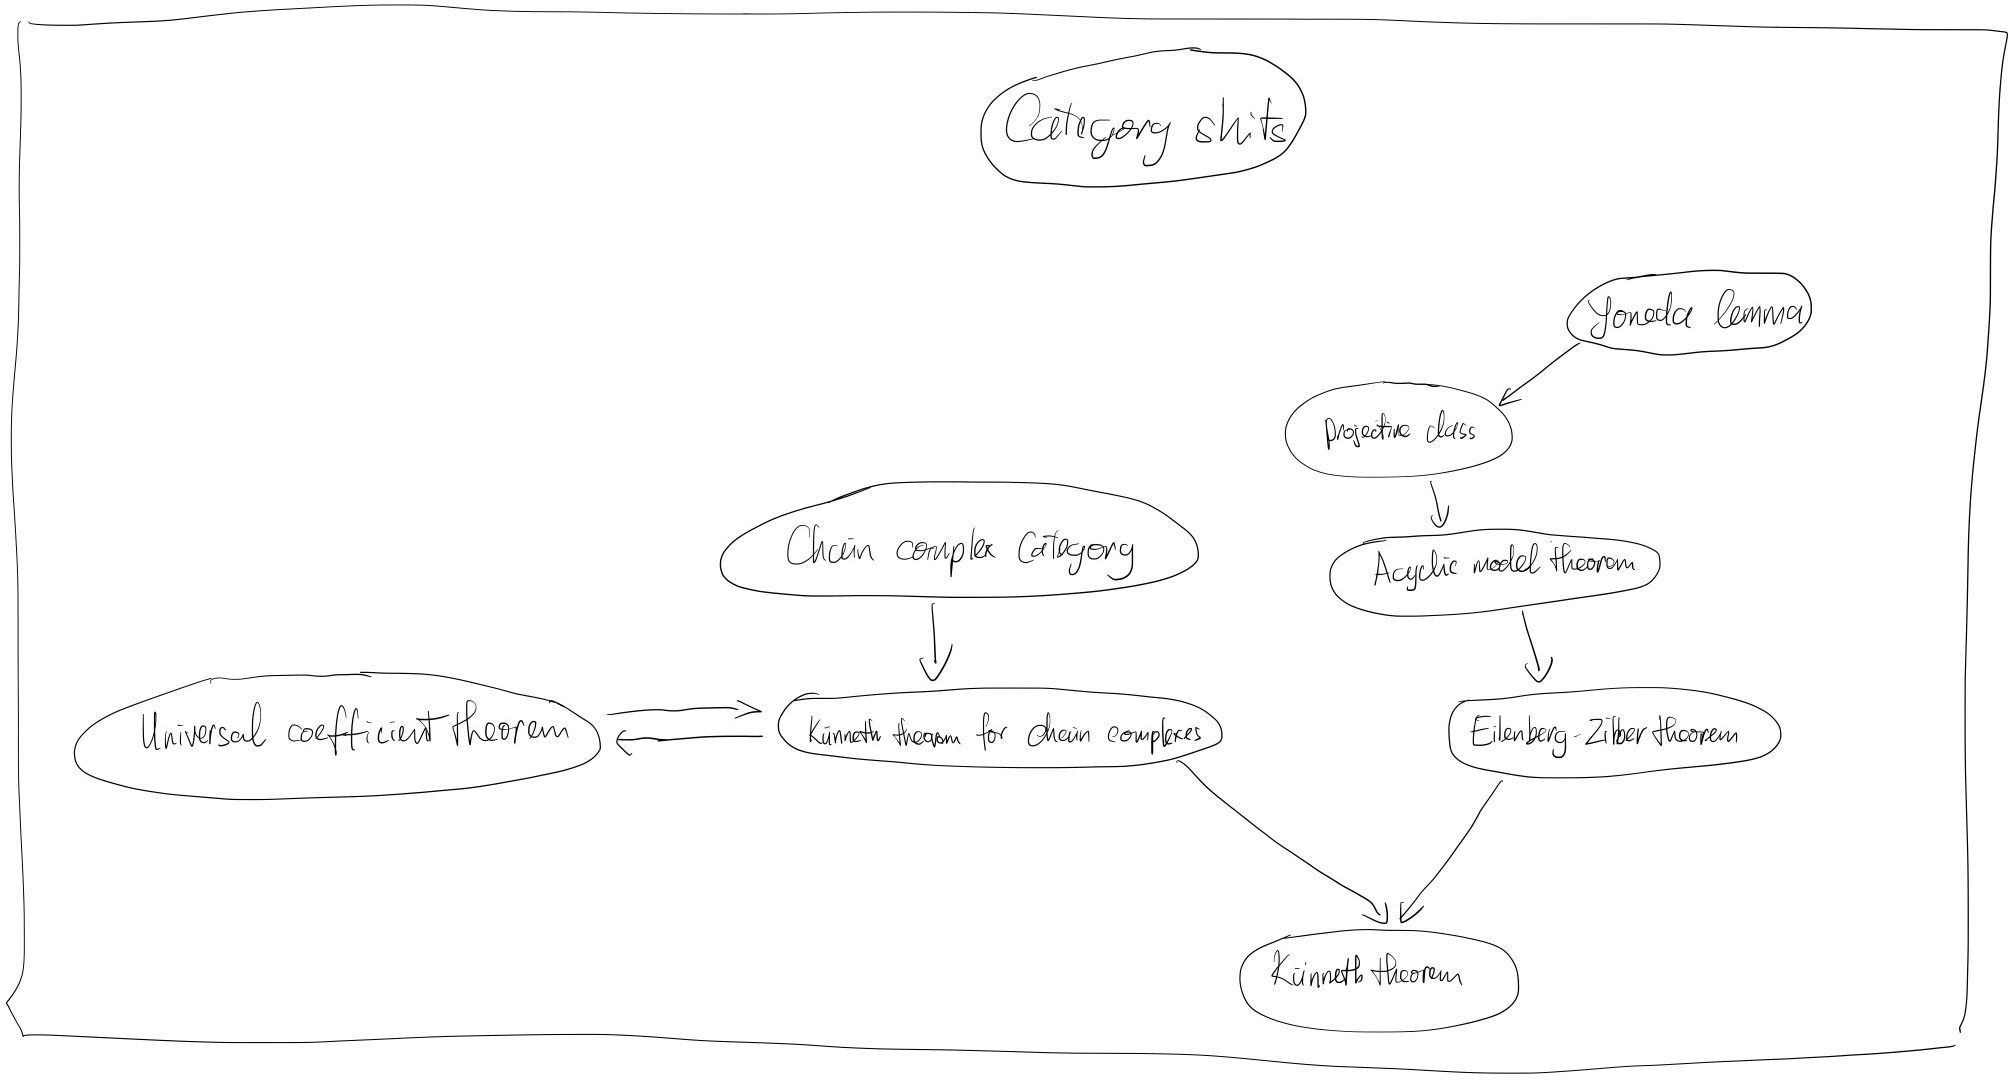
\includegraphics[width=0.8\textwidth]{roadmap.jpg}
        \caption{road map}
        \label{fig:roadmap}
    \end{figure}
\end{center}

\section{UNIVERSAL COEFFICIENT THEOREM}

\begin{theorem}[universal coefficient theorem]
    Let $R$ be a PID, $N$ be an $R$-module, $C_\bullet$ be chain complexes of $R$-module, and $C_\bullet$ is degree-wise free (each $C_n$ is a free $R$-module). Then, there is a short exact sequence
    \begin{center}
        \begin{tikzcd}
        0 \arrow[r] & H_n(C_\bullet) \otimes N \arrow[rr] &  & H_n(C_\bullet \otimes N) \arrow[rr] &  & {\Tor_1(H_{n-1}(C_\bullet), N)} \arrow[r] & 0
        \end{tikzcd}
    \end{center}
    and this sequence splits (but not naturally)
\end{theorem}

\section{KÜNNETH THEOREM FOR CHAIN COMPLEXES OF $R$-MODULES}

\begin{definition}[direct sum of chain complexes of $R$-module]
    In the category of chain complexes of $R$-module ($\Ch(\RMod)$), let $C_\bullet, D_\bullet \in \ob \Ch(\RMod)$, define the direct sum $C_\bullet \oplus D_\bullet \in \ob \Ch(\RMod)$ as follows:
    $$
        (C_\bullet \oplus D_\bullet)_n = C_n \oplus D_n
    $$
    and the boundary map $\partial: (C_\bullet \oplus D_\bullet)_n \to (C_\bullet \oplus D_\bullet)_{n-1}$ is defined by
    \begin{align*}
        \partial:   (C \oplus D)_n &\to (C \oplus D)_{n-1} \\
                    c \oplus d &\mapsto \partial c \oplus \partial d
    \end{align*}
    
\end{definition}

\begin{definition}[tensor product of chain complexes of $R$-module]
    In the category of chain complexes of $R$-module ($\Ch(\RMod)$), let $C_\bullet, D_\bullet \in \ob \Ch(\RMod)$, define the tensor product $C_\bullet \otimes D_\bullet \in \ob \Ch(\RMod)$ as follows:
    $$
        (C_\bullet \otimes D_\bullet)_n = \bigoplus_{p + q = n} C_p \otimes D_q
    $$
    and the boundary map $\partial: (C_\bullet \otimes D_\bullet)_n \to (C_\bullet \otimes D_\bullet)_{n-1}$ is the linear extension of $\partial: C_p \otimes D_q \to (C_\bullet \otimes D_\bullet)_{n-1}$ where
    $$
        \partial (c \otimes d) = \partial c \otimes d + (-1)^{|c|} c \otimes \partial d
    $$
    where $c \otimes d \in C_p \otimes D_q$ and $|c| = p$
\end{definition}

\begin{proof}
    \note{TODO - bilinear chain map factors through tensor product}
\end{proof}

\begin{definition}[the $\Tor$ functor]
    \note{TODO}
\end{definition}

\begin{theorem}[Künneth theorem for chain complexes]
    Let $R$ be a PID, $C_\bullet, D_\bullet$ be chain complexes of $R$-module, and $C_\bullet$ is degree-wise free (each $C_n$ is a free $R$-module). Then, there is a short exact sequence
    \begin{center}
        \begin{tikzcd}
        0 \arrow[r] & \bigoplus_{p+q=n} H_p(C_\bullet) \otimes H_q(D_\bullet) \arrow[r, "\times"] & H_n(C_\bullet \otimes D_\bullet) \arrow[r] & {\bigoplus_{p+q=n-1} \Tor^R_1 (H_p(C_\bullet), H_q(D_\bullet))} \arrow[r] & 0
        \end{tikzcd}
    \end{center}
    and this sequence splits (but not naturally)
\end{theorem}

\begin{proof}
    Consider the case where the boundary map in $C_\bullet$ is zero, that is, for all $c \in C_n$, $\partial c = 0$. Then, 
    \begin{align*}
        \partial:   C_p \otimes D_q &\to C_p \otimes D_{q-1} \\
                    c \otimes d &\mapsto (-1)^{|c|} c \otimes \partial d
    \end{align*}
    
    Hence, $C_\bullet \otimes D_\bullet$ can be written as a direct sum of chain complexes $C_\bullet \otimes D_\bullet = \bigoplus_p C_p \otimes D_{\bullet-p}$. Therefore
    \begin{align*}
        H_n(C_\bullet \otimes D_\bullet) 
        &= H_n\tuple*{\bigoplus_p C_p \otimes D_{\bullet-p}} \\
        &= \bigoplus_p H_n(C_p \otimes D_{\bullet-p}) \\
        &= \bigoplus_p C_p \otimes H_n(D_{\bullet - p}) &\text{($C_p$ is free, cons of UCT)}\\
        &= \bigoplus_{p + q = n} C_p \otimes H_q(D_\bullet)&\text{(shifted chain complex)}\\
        &= \bigoplus_{p + q = n} H_p(C_\bullet) \otimes H_q(D_\bullet) &\text{($C_p = H_p(C_\bullet)$)}
    \end{align*}

    Now let $C_\bullet$ be an arbitrary chain complex, we have the short exact sequence of chain complexes
    \begin{center}
        \begin{tikzcd}
        0 \arrow[r] & Z_\bullet \arrow[r] & C_\bullet \arrow[r] & B_{\bullet -1} \arrow[r] & 0
        \end{tikzcd}
    \end{center}

    where $Z_n = \ker(\partial: C_n \to C_{n-1})$ and $B_n = \im (\partial: C_{n+1} \to C_n)$ are $n$-cycle and $n$-boundary and consider $Z_\bullet, B_{\bullet-1}$ as chain complexes with zero boundary map. Each $Z_n, B_n$ are free as they are submodules of free $R$-module $C_n$. As $B_{\bullet - 1}$ is free, the sequence splits, hence, the sequence below is exact
    \begin{center}
        \begin{tikzcd}
        0 \arrow[r] & Z_\bullet \otimes D_\bullet \arrow[r] & C_\bullet \otimes D_\bullet \arrow[r] & B_{\bullet -1} \otimes D_\bullet \arrow[r] & 0
        \end{tikzcd}
    \end{center}
    
    That induces a long exact sequence in homology
    \begin{center}
        \begin{tikzcd}
                                                       & ... \arrow[r]                              & H_{n+1}(B_{\bullet-1} \otimes D_\bullet) \arrow[lld, "(i_n)_*"'] \\
        H_n(Z_\bullet \otimes D_\bullet) \arrow[r]     & H_n(C_\bullet \otimes D_\bullet) \arrow[r] & H_n(B_{\bullet-1} \otimes D_\bullet) \arrow[lld, "(i_{n-1})_*"'] \\
        H_{n-1}(Z_\bullet \otimes D_\bullet) \arrow[r] & ...                                        &                                                                 
        \end{tikzcd}
    \end{center}

    where the connecting homomorphisms $(i_n)_*, (i_{n-1})_*$ are induced by inclusion maps

    \begin{center}
        \begin{tikzcd}
                                        &                                                 & (B_{\bullet-1} \otimes D_\bullet)_{n+1} \arrow[lld, "i_n"'] \arrow[ld, hook] \\
        (Z_\bullet \otimes D_\bullet)_n & (C_\bullet \otimes D_\bullet)_n \arrow[l, hook] &                                                                           
        \end{tikzcd}
    \end{center}

    From the long exact sequence, we have the short exact sequence
    \begin{center}
        \begin{tikzcd}
        0 \arrow[r] & \coker(i_n)_* \arrow[r] & H_n(C_\bullet \otimes D_\bullet) \arrow[r] & \ker(i_{n-1})_* \arrow[r] & 0
        \end{tikzcd}
    \end{center}

    Discussed in the previous argument, as $Z_\bullet$ and $B_{\bullet-1}$ are free,

    \begin{align*}
        H_n(Z_\bullet \otimes D_\bullet) &= \bigoplus_{p + q = n} Z_p \otimes H_q(D_\bullet) \\
        H_{n+1}(B_{\bullet-1} \otimes D_\bullet) &= \bigoplus_{p + q = n} B_p \otimes H_q(D_\bullet)
    \end{align*}

    Since tensor product is right-exact, exactness of the top sequence implies exactness of the bottom sequence
    \begin{center}
        \begin{tikzcd}
        0 \arrow[r] & B_p \arrow[rr, "j", hook]                                            &  & Z_p \arrow[rr, two heads]                        &  & H_p(C_\bullet) \arrow[r]                        & 0 \\
                    & B_p \otimes H_q(D_\bullet) \arrow[rr, "(i_*)_{p+q} = j \otimes 1", hook] &  & Z_p \otimes H_q(D_\bullet) \arrow[rr, two heads] &  & H_p(C_\bullet) \otimes H_q(D_\bullet) \arrow[r] & 0
        \end{tikzcd}
    \end{center}

    Hence, $\coker(i_*)_n = \bigoplus_{p + q = n} H_p(C_\bullet) \otimes H_p(D_\bullet)$. On the other hand, the top sequence is the free resolution of $H_p(C_\bullet)$. Then, $\Tor^R_1(H_p(C_\bullet), H_q(D_\bullet))$ is the first homology group of the bottom sequence
    \begin{center}
        \begin{tikzcd}
        2           & 1                                                                    &  & 0                                     &  &   \\
        0 \arrow[r] & B_p \arrow[rr, "j", hook]                                            &  & Z_p \arrow[rr]                        &  & 0 \\
        0 \arrow[r] & B_p \otimes H_q(D_\bullet) \arrow[rr, "(i_*)_{p+q} = j \otimes 1", hook] &  & Z_p \otimes H_q(D_\bullet) \arrow[rr] &  & 0
        \end{tikzcd}
    \end{center}

    That is, $\ker(i_*)_{n-1} = \bigoplus_{p + q = n-1} \Tor^R_1(H_p(C_\bullet), H_q(D_\bullet))$

    \note{TODO - here, there are to functors, one is $\otimes D$ composed with $H$ and the other is $\otimes H(D)$ - need to prove }

    \note{TODO - split}
\end{proof}










\section{KÜNNETH THEOREM FOR TOPOLOGICAL SPACES}

\subsection{FUNDAMENTAL THEOREM OF HOMOLOGICAL ALGEBRA}

\begin{definition}[initial object, terminal object, pointed category, zero map, kernel]
    Given a category $C$, an object $0$ is initial if for all $X \in \ob C$, there is only one map in $\Hom(0, X)$, an object $*$ is terminal if for all $X \in \ob C$, there is only one map in $\Hom(X, *)$. Category $C$ is called pointed if it has initial and terminal objects and the unique map $0 \to *$ is an isomorphism.
    
    If $C$ is a pointed category, we use the same symbol $0$ for both initial object and terminal object. There exists a zero map between any two objects $M, N \in \ob C$, defined by
    \begin{center}
        \begin{tikzcd}
        M \arrow[r] \arrow[rd, "0"'] & 0 \arrow[d] \\
                                     & N          
        \end{tikzcd}
    \end{center}
    the composition of $M \to 0$ and $0 \to N$. Let $f: M \to N$ be a morphism in $C$, a kernel of $f$ is a map $i: K \to M$ such that $f i = 0$ and such map is universal, that is, if $j: L \to M$ with $f j = 0$, then it factors through $K$
    \begin{center}
        \begin{tikzcd}
        K \arrow[r, "i"] \arrow[rr, "0", bend left=49]                     & M \arrow[r, "f"] & N \\
        L \arrow[ru, "j"'] \arrow[u, dashed] \arrow[rru, "0"', bend right] &                  &  
        \end{tikzcd}
    \end{center}
    Category $C$ has kernels if every morphism has a kernel.
\end{definition}

\begin{definition}[preadditive category, $\Ab$-enriched category]
    A category $C$ is called preadditive category (or $\Ab$-enriched category) if for any two objects $M, N \in \ob C$, $\Hom(M, N)$ is an abelian group and composition is bilinear, that is, if $f, g, h$ are morphisms in $C$
    \begin{align*}
        f (g + h) = fg + fh \\
        (f + g) h = fh + gh
    \end{align*}
\end{definition}

\begin{definition}[chain complex, acyclic chain complex, exact sequence]
    In a pointed category with kernels, a chain complex is a sequence such that given any subsequence $A \to B \to C$, $A \to B$ factors through $\ker (B \to C)$, that is, there exists a map $A \to \ker (B \to C)$ such that the diagram below commutes
    \begin{center}
    \begin{tikzcd}
    ... \arrow[r] & A \arrow[r] \arrow[d, dashed] & B \arrow[r] & C \arrow[r] & ... \\
                  & \ker (B \to C) \arrow[ru]     &             &             &    
    \end{tikzcd}
    \end{center}

    If there is a notion of epimorphism and the map $A \to \ker (B \to C)$ is an epimorphism, then the sequence is called exact at $B$. A sequence is called exact sequence or an acyclic chain complex if it is exact everywhere, possibly except the two ends.
\end{definition}

\begin{definition}[chain map, chain homotopy]
    Given two chain complexes $C_\bullet, D_\bullet$ in a pointed category with kernels, for each $n \in \Z$, there is a map $f_n: C_n \to D_n$ such that the diagram below commutes, then $f_\bullet$ is called a chain map
    \begin{center}
    \begin{tikzcd}
    ... & C_{n-1} \arrow[l] \arrow[d, "f_{n-1}"] & C_n \arrow[l] \arrow[d, "f_n"] & C_{n+1} \arrow[l] \arrow[d, "f_{n+1}"] & ... \arrow[l] \\
    ... & D_{n-1} \arrow[l]                      & D_n \arrow[l]                  & D_{n+1} \arrow[l]                      & ... \arrow[l]
    \end{tikzcd}
    \end{center}

    Chain complexes and chain maps form a category and it is called the category of chain complexes.

    Given two chain complexes $C_\bullet, D_\bullet$ in a pointed \textbf{preadditive} category with kernels. Let $f_\bullet, g_\bullet: C_\bullet \to D_\bullet$ be two chain maps. A chain homotopy from $f_\bullet$ to $g_\bullet$ is a collection of maps $h_n: C_{n-1} \to D_n$ such that $\partial h_{n+1} + h_n \partial = f_n - g_n$

    \begin{center}
    \begin{tikzcd}
    ... & C_{n-1} \arrow[l, "\partial"'] \arrow[rd, "h_n"] & C_n \arrow[l, "\partial"'] \arrow[rd, "h_{n+1}"] & C_{n+1} \arrow[l, "\partial"'] & ... \arrow[l, "\partial"'] \\
    ... & D_{n-1} \arrow[l, "\partial"]                    & D_n \arrow[l, "\partial"]                        & D_{n+1} \arrow[l, "\partial"]  & ... \arrow[l, "\partial"] 
    \end{tikzcd}
    \end{center}
    
    
\end{definition}

\begin{definition}[projective class]
    Let $C$ be a pointed category with kernels. A projective class in $C$ is a pair $(\mathcal{P}, \mathcal{E})$ where $\mathcal{P}$ is a collection of objects (called \textbf{projectives}) and $\mathcal{E}$ is a collection of morphisms (called \textbf{epimorphisms}) such that
    \begin{enumerate}
        \item An object $P$ is \textbf{projective} if and only if $P$ has the universal lifting property against every \textbf{epimorphism} $M \to N$, that is, given any \textbf{epimorphism} $M \to N$, if there is a map $P \to N$, then it factors through $M$
        \begin{center}
            \begin{tikzcd}
            M \arrow[r, "epi", two heads] & N                              \\
                                          & P \arrow[lu, dashed] \arrow[u]
            \end{tikzcd}
        \end{center}

        \item A morphism $f: M \to N$ is an \textbf{epimorphism} if and only if every \textbf{projective} has the universal lifting property against $f$, that is, given any \textbf{projective} $P$, if there is a map $P \to N$, then it factors through $M$

        \begin{center}
            \begin{tikzcd}
            M \arrow[r, "f", two heads] & N                              \\
                                          & P \arrow[lu, dashed] \arrow[u]
            \end{tikzcd}
        \end{center}

        \item $C$ has enough \textbf{projectives}, that is, given any object $M \in \ob C$, for every \textbf{projective} $P$, there exists an \textbf{epimorphism} $P \to M$.
    \end{enumerate}
\end{definition}



\begin{theorem}[fundamental theorem of homological algebra]
    Let $C$ be a pointed category with kernels and $(\mathcal{P}, \mathcal{C})$ be a projective class in $C$. Given $f: M \to M'$ in $C$ and the diagram below
    \begin{center}
        \begin{tikzcd}
        0 & M \arrow[l] \arrow[d, "f"] & P_0 \arrow[l, "\epsilon"'] \arrow[d, "f_0", dashed] & P_1 \arrow[l, "d"'] \arrow[d, "f_1", dashed] & ... \arrow[l, "d"']  \\
        0 & M' \arrow[l]               & P'_0 \arrow[l, "\epsilon'"']                        & P'_1 \arrow[l, "d'"']                        & ... \arrow[l, "d'"']
        \end{tikzcd}
    \end{center}

    where both chains are chain complexes, the top chain consists of projectives $P_n$ and the bottom chain is acyclic. Then,
    \begin{itemize}
        \item There exists a chain map defined by $f_n: P_n \to P'_n$
        \item If $C$ is preadditive, the lift is unique upto chain homotopy.
    \end{itemize}
\end{theorem}

\begin{longproof}
    \begin{enumerate}
        \item The first statement is proved by induction
        \begin{center}
        \begin{tikzcd}
        P_{n-2} \arrow[dd, "f_{n-2}"'] & P_{n-1} \arrow[l] \arrow[dd, "f_{n-1}"'] &                     & P_n \arrow[dd, "f_n", dashed] \arrow[ll] \arrow[ld, dashed] \\
                                       &                                          & K'_{n-1} \arrow[ld] &                                                             \\
        P'_{n-2}                       & P'_{n-1} \arrow[l]                       &                     & P'_n \arrow[lu, two heads] \arrow[ll]                      
        \end{tikzcd}
        \end{center}

        Suppose there exist maps $f_{n-1}: P_{n-1} \to P'_{n-1}$ and $f_{n-2}: P_{n-2} \to P'_{n-2}$. Let $K'_{n-1} = \ker(P'_{n-1} \to P'_{n-2})$.
        
        Since the bottom chain is acyclic, the map $P'_n \to P'_{n-1}$ factors through $K'_{n-1}$ by an epimorphism.

        Since the top chain is a chain complex, the composition $P_n \to P_{n-1} \to P'_{n-1} \to P'_{n-2}$ equals $P_n \to P_{n-1} \to P_{n-2} \to P'_{n-2}$ and equals 0 zero, so $P_n \to P_{n-1} \to P'_{n-1}$ factors through $K'_{n-1}$

        Since $P_n$ is projective and $P'_n \to K'_{n-1}$ is an epimorphism, $P_n \to K'_{n-1}$ factors through $P'_n$ by a map $f_n: P_n \to P'_n$

        \textbf{Base case}: $n=0$, let $P_{n-1} = M, P'_{n-1} = M'$, $P_{n-2} = 0, P'_{n-2} = 0$ and $f_{n-1} = f, f_{n-2} = 0$
        
        \item Let $f^{(1)}_\bullet, f^{(2)}_\bullet: P_\bullet \to P'_\bullet$ be any two lifts from $f: M \to M'$

        \begin{center}
        \begin{tikzcd}
        M \arrow[d, "f"'] & P_\bullet \arrow[l, "\epsilon"] \arrow[d, "f^{(1)}_\bullet"', dashed, bend right] \arrow[d, "f^{(2)}_\bullet", dashed, bend left] \\
        M'                & P'_\bullet \arrow[l, "\epsilon'"]                                                                                                
        \end{tikzcd}
        \end{center}

        We will prove that $g_\bullet = f^{(1)}_\bullet - f^{(2)}_\bullet$ is chain homotopic to zero, that is to find maps $h_{n+1}: P_n \to P'_{n+1}$ such that $d'h + hd = g$

        \begin{center}
        \begin{tikzcd}
        0 \arrow[d, "0"'] & P_0 \arrow[l, "d"'] \arrow[d, "g_0"'] & P_1 \arrow[l, "d"'] \arrow[d, "g_1"'] & ... \arrow[l, "d"'] \\
        0                 & P'_0 \arrow[l, "d'"]                  & P'_1 \arrow[l, "d'"]                  & ... \arrow[l, "d'"]
        \end{tikzcd}
        \end{center}

        Suppose there exists map $h_{n-1}: P_{n-2} \to P'_{n-1}$ and $h_{n-2}: P_{n-3} \to P'_{n-2}$ such that
        $$
            g_{n-2} - h_{n-2} d = d' h_{n-1}
        $$

        \begin{center}
        \begin{tikzcd}
        P_{n-3} \arrow[rrdd, "h_{n-2}"] &  & P_{n-2} \arrow[rrdd, "h_{n-1}"] \arrow[ll, "d"'] &  & P_{n-1} \arrow[ll, "d"']  \\
                                        &  &                                                  &  &                           \\
        P'_{n-3}                        &  & P'_{n-2} \arrow[ll, "d'"]                        &  & P'_{n-1} \arrow[ll, "d'"]
        \end{tikzcd}
        \end{center}

        Consider the map $g_{n-1} - h_{n-1} d: P_{n-1} \to P'_{n-1}$,
        \begin{align*}
            d'(g_{n-1} - h_{n-1} d) 
            &= d' g_{n-1} - d' h_{n-1} d &\text{(preadditive)}\\
            &= d' g_{n-1} - (g_{n-2} - h_{n-2} d) d &\text{(induction)}\\
            &= d' g_{n-1} - g_{n-2} d &\text{(preadditive, $dd=0$)}\\
            &= 0 &\text{($g_\bullet$ is a chain map)}
        \end{align*}

        Let $K'_{n-1} = \ker(d': P'_{n-1} \to P'_{n-2})$.

        Since the bottom chain is acyclic, the map $d': P'_n \to P'_{n-1}$ factors through $K'_{n-1}$ by an epimorphism.

        \begin{center}
\begin{tikzcd}
P_{n-2} \arrow[rrdd, "h_{n-1}"] &  & P_{n-1} \arrow[ll, "d"'] \arrow[d, dashed] \arrow[rrdd, "h_n", dashed] &  &                                                      \\
                                &  & K'_{n-1} \arrow[d]                                                     &  &                                                      \\
P'_{n-2}                        &  & P'_{n-1} \arrow[ll, "d'"]                                              &  & P'_n \arrow[llu, two heads, dashed] \arrow[ll, "d'"]
\end{tikzcd}
        \end{center}

        As $d'(g_{n-1} - h_{n-1} d) = 0$, $g_{n-1} - h_{n-1} d$ factors through $K'_{n-1}$, that is, $g_{n-1} - h_{n-1} d$ equals the composition $P_{n-1} \to K'_{n-1} \to P'_{n-1}$

        Since $P_{n-1}$ is projective and $P'_n \to K'_{n-1}$ is an epimorphism, $P_{n-1} \to K'_{n-1}$ factors through $P'_n$ by a map $h_n: P_{n-1} \to P'_n$, that is, the $d' h_n$ equals the composition $P_{n-1} \to P'_n \to K'_{n-1} \to P'_{n-1}$ and equals the composition $P_{n-1} \to K'_{n-1} \to P'_{n-1}$, hence

        $$
            d' h_n = g_{n-1} - h_{n-1} d
        $$

        \textbf{Base case}: $n=0$, let $P_{n-2} = 0, P'_{n-2} = 0$, $P_{n-1} = M, P'_{n-1} = M'$, $h_{n-1} = 0$, then 
        \begin{align*}
            d'(g_{n-1} - h_{n-1} d) 
            &= 0 &\text{($d': P'_{n-1} \to P'_{n-2}$ is the zero map $M' \to 0$)}
        \end{align*}
        
    \end{enumerate}
\end{longproof}

\subsection{RESOLUTION AND TOR FUNCTOR}

\begin{definition}[resolution, projective resolution]
    Let $M$ be an object in a pointed category with kernels. A resolution of $M$ is an exact sequence
    \begin{center}
    \begin{tikzcd}
    0 & M \arrow[l] & P_0 \arrow[l, "\epsilon"'] & P_1 \arrow[l, "d"'] & ... \arrow[l, "d"']
    \end{tikzcd}
    \end{center}

    If $P_n$ are projectives in a projective class $(\mathcal{P}, \mathcal{E})$, then the sequence is called $\mathcal{P}$-projective resolution.
\end{definition}

\begin{corollary}
    Let $M$ be an object in a pointed preadditive category with kernels. Any two projective resolutions of $M$ are chain homotopy equivalent \footnote{two chain complexes $C_\bullet, D_\bullet$ are chain homotopy equivalent if there are two chain maps $f_\bullet: C_\bullet \to D_\bullet$, $g_\bullet: D_\bullet \to C_\bullet$ such that $gf$ and $fg$ are chain homotopic to identity} or equivalently $M$ defines a chain homotopy type.
\end{corollary}

\begin{definition}[Tor functor on $\RMod$]
    \note{TODO}
\end{definition}



\subsection{EILENBERG-ZILBER THEOREM}


\begin{proposition}[projective module, projective class in $\RMod$]
    In the category of $R$-module ($\RMod$), there is a projective class $(\mathcal{P}, \mathcal{E})$ defined by epimorphism being surjective homomorphism. Then, the following are equivalent
    \begin{enumerate}
        \item $P \in \ob \RMod$ is projective
        \item Every short exact sequence $0 \to M \to N \to P \to 0$ splits
        \item $P$ is a direct summand of a free $R$-module, that is, there exists $Q \in \ob \RMod$ such that $P \oplus Q$ is a free $R$-module.
    \end{enumerate}    
\end{proposition}

\begin{proof}
    \note{TODO}
\end{proof}

\begin{proposition}[models define projective class in $\Fun(C, \RMod)$]
    Given a category $C$, $\Fun(C, \RMod)$ is a pointed preadditive category with kernels (more precisely, abelian category - will define in the future).

    Let $\mathcal{M}$ be any set of objects in $C$ (called models), then $\mathcal{M}$ defines a projective class $(\mathcal{P}, \mathcal{E})$ in $\Fun(C, \RMod)$ where a morphism $G \to F$ is an epimorphism (relative to $\mathcal{M}$) if for all $M \in \mathcal{M}$, $G(M) \twoheadrightarrow F(M)$ is surjective. Then, the following are equivalent
    
    \begin{enumerate}
        \item $P \in \ob \Fun(C, \RMod)$ is projective
        \item $P$ is a \textbf{retract of coproduct} of $R \Hom(M, -)$ for some $M \in \mathcal{M}$ where $\Hom(M, -)$ is a functor $\RMod \to \Set$, $R$ is the free $R$-module functor $\Set \to \RMod$. In the case of $R$-module, \textbf{retract of coproduct} is the \textbf{direct summand} of a $R$-module
    \end{enumerate}
\end{proposition}

\begin{proof}
    \note{TODO - prove using Yoneda lemma}
\end{proof}

\begin{theorem}[Eilenberg-Zilber theorem]
    \note{TODO}
\end{theorem}







\end{document}
